\section{Results}

\begin{figure}[h]
  \includegraphics[width=\linewidth]{tileset_rrti.png}
  \caption{a) The exemplar image, take from Wo\'zniak's Forest Micro tile set with a single tile highlighted in red with it's neighbors, as they appear in
           the exemplar image highlighted in orange.
           b) The inferred tile set, packed into an image with the highlighted tile in red and its neighbor tiles highlighted in orange. Note that even though
           tiles in the tile set might look the same, these represent different tiles as they have different constraints for which neighbors are permissible.
           c) A catalog of super tiles, with the highlighted tile in red and its neighbors highlighted in orange. Each super tile consists of a 2x2 window
           taken from the exemplar image (a). Neighbors are derived from the corresponding overlap of the 2x1 tile window  for left and right neighbors and
           a 1x2 tile window for the up and down neighbors. Grey regions represent tiles that fall outside of the exemplar image. }
  \label{fig:rrti_tileset}
\end{figure}

\begin{figure*}[ht]
  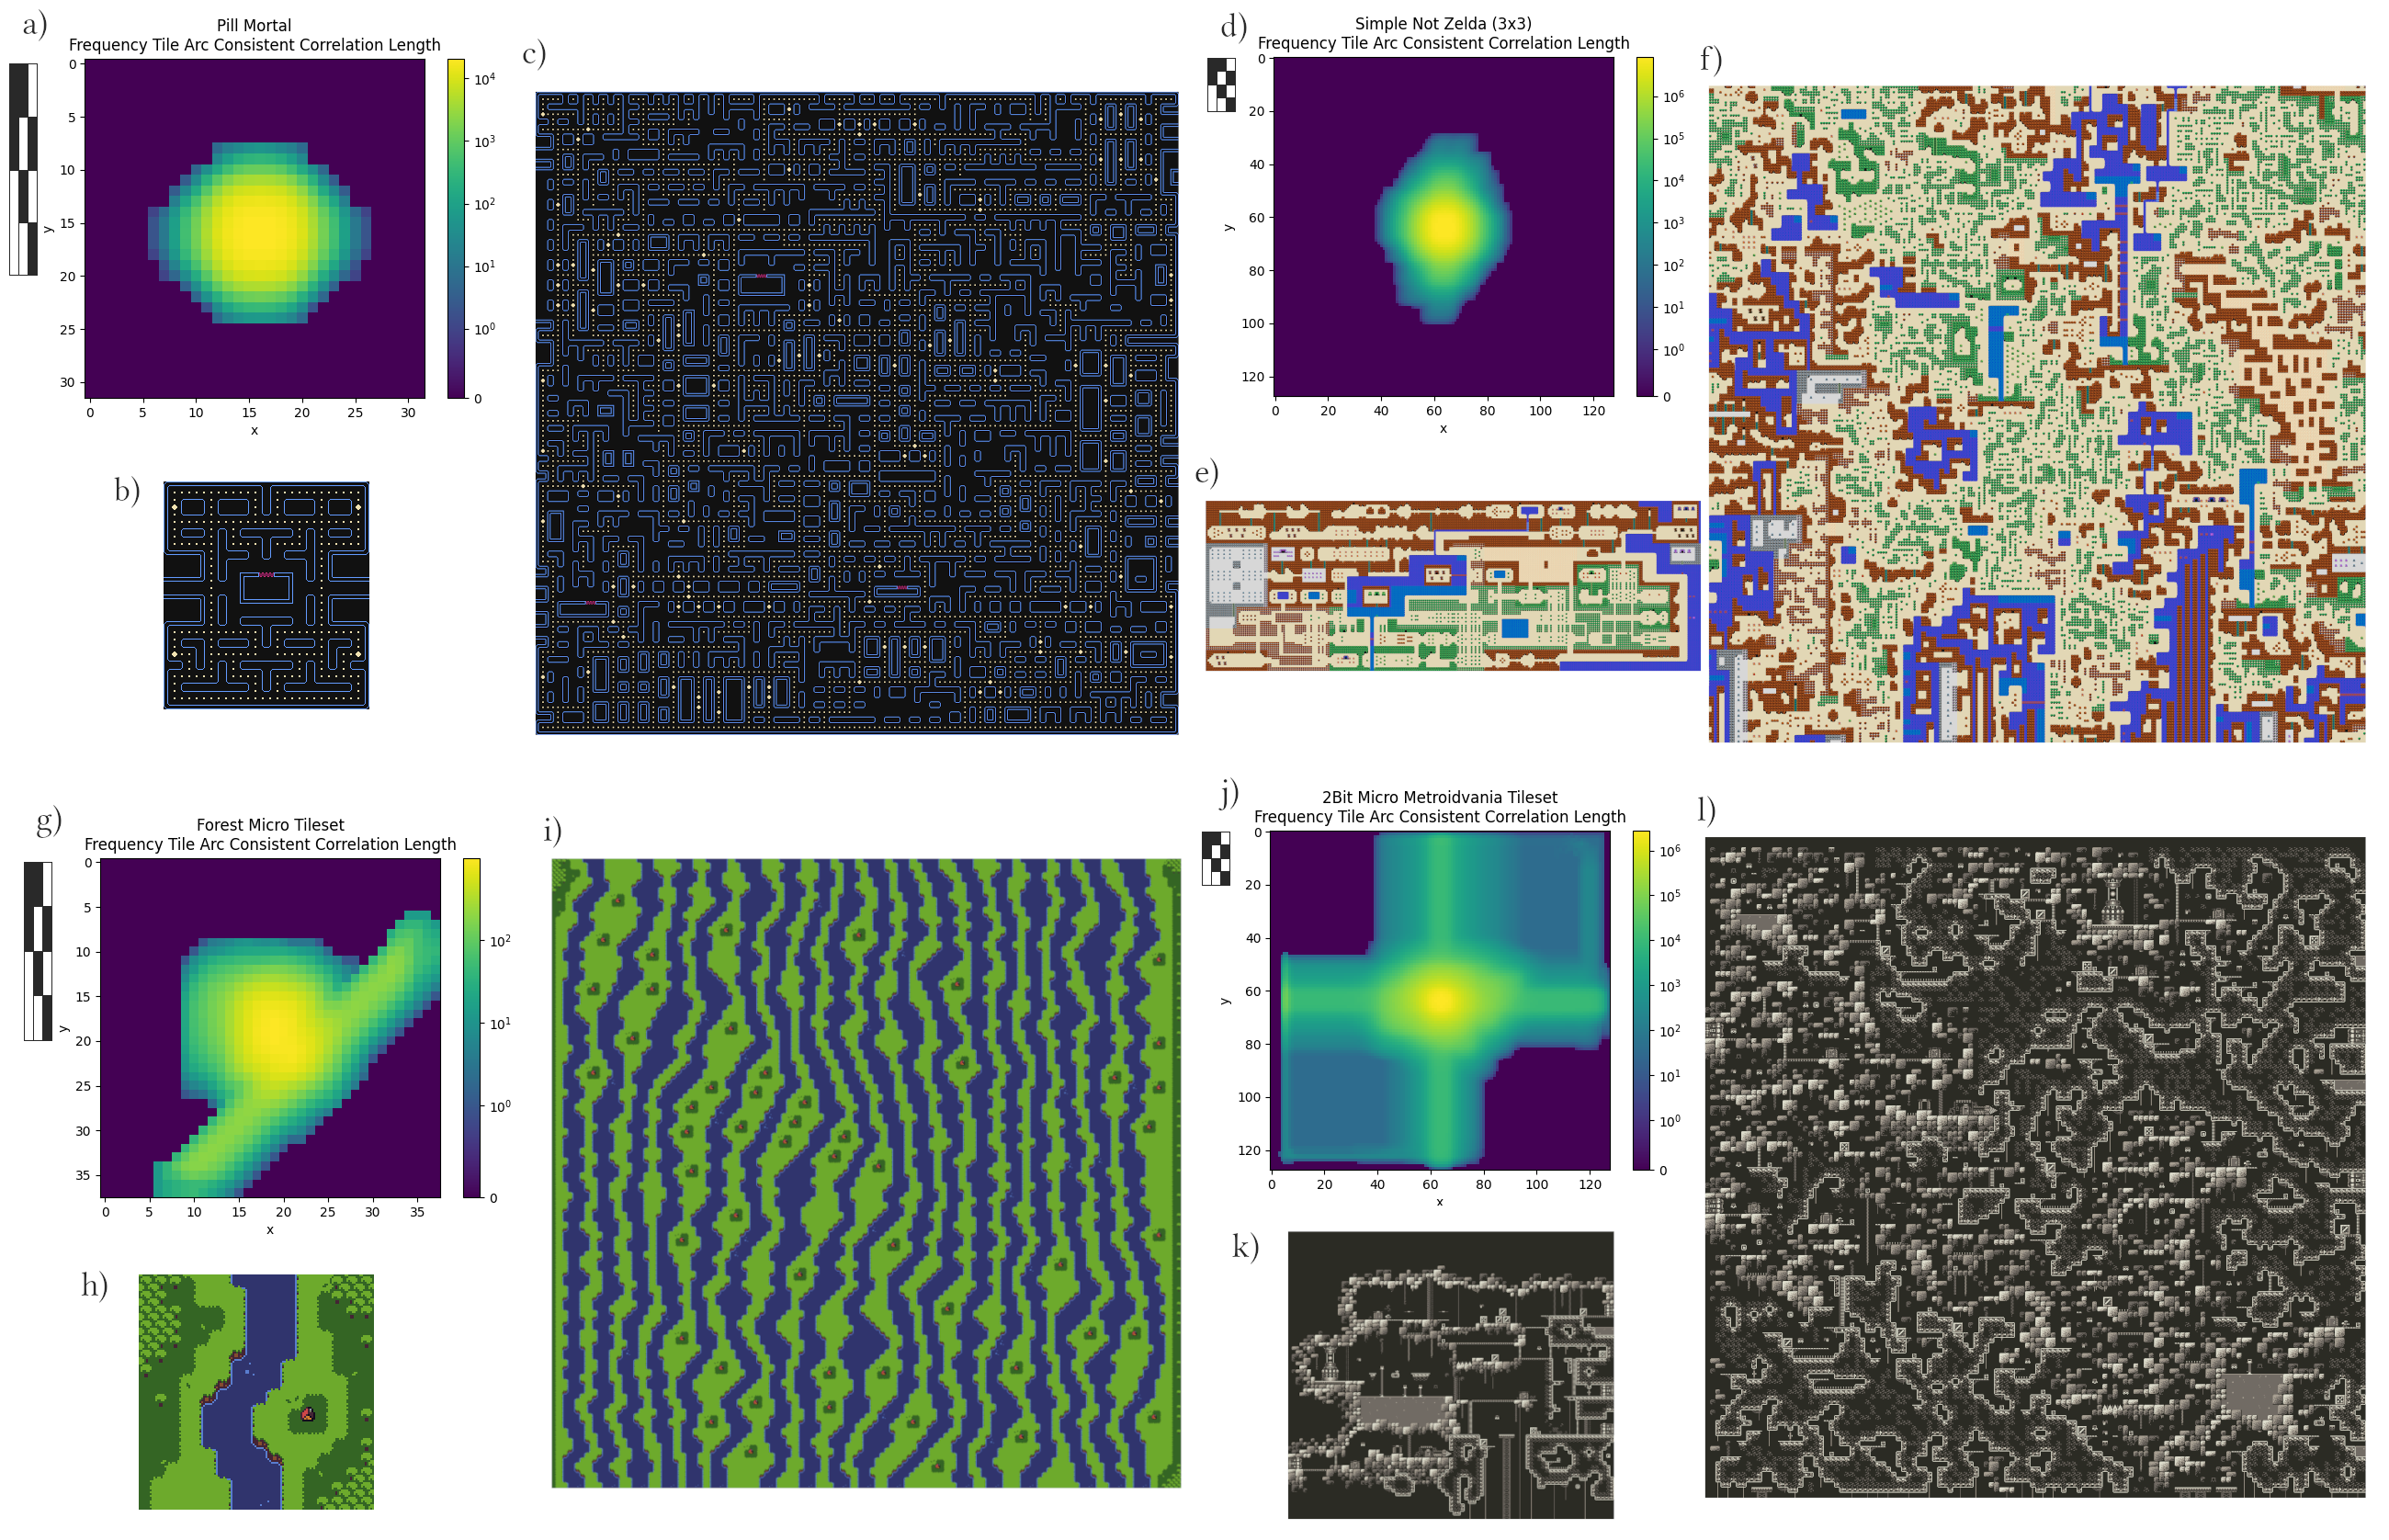
\includegraphics[width=\textwidth]{2d_poms_examples.png}
  \caption{Tile Arc Consistent Correlation Length (TACCL) plots, source exemplar image and example output for four 2D tile sets as listed in Table \ref{table:tilesets}.
           The TACCL, exemplar image and example 64x64 output using a block size of 8x8 for the \textit{Pill Mortal} tile set are shown in a), b) and c) respectively. The TACCL, exemplar image and an example 256x256 output using a block size of 50x70 for LUNARSIGNALS' \textit{Overhead Action RPG Overworld} are shown in d), e) and f) respectively. The TACCL, exemplar image and an example 128x128 output using a block size of 48x48 for Wo\'zniak's \textit{Forest Micro} tile set are shown in g), h) and i) respectively. The TACCL, exemplar image and an example 128x128 output using a block size of 48x48 for 0x72's \textit{Two Bit Micro Metroidvania} tile set are shown in j), k), l) respectively. }
  \label{fig:2dexamples}
\end{figure*}

\begin{figure}[h]
  \centering
  \includegraphics[width=\linewidth]{brutal-plum_cons.png}
  \caption{The Tile Arc Consistent Correlation Length (TACCL) plot, source tile set and an example 32x32x32 output for the 3d \textit{Brutal Plum} tile set listed in a), b) and c) respectively. A block size of 22x22x22 was used.}
  \label{fig:brutal_plum}
\end{figure}

In this section, we highlight five tile sets that represent different aspects of the
benefits and pitfalls of the Punch Out Model Synthesis (POMS) algorithm.

The four 2D tile sets had their tile constraints inferred from an exemplar image using
an automated tile constraint generation method.
The exemplar image is split into tiles and a sliding super tile window, of a larger size than the tile itself, is moved over the exemplar image.
The super tiles are deduplicated and checked for overlapping bands to other super tiles.
For every matching, overlapping band, a constraint is added to the tile constraints, allowing an admissible pairing for the tiles in the
appropriate dimension direction.

Figure \ref{fig:rrti_tileset} shows the exemplar image (\textit{a}), the inferred tile set (\textit{b}) and the complete list of super tiles
for Wo\'zniak's \textit{Forest Micro} tile set.
A single tile is highlighted in red and its neighbors are highlighted in yellow with red edges corresponding to their neighboring direction.

Figure \ref{fig:rrti_tileset} uses a tile size of 8x8 pixels, with a 2x2 super tile size.
The upper left hand tile is used as the displayed representative tile, which can be seen by comparing the non dimmed tiles in the
super tile list from Figure \ref{fig:rrti_tileset} (\textit{c}) to the packed tile set image (\textit{b}).
A 2x1 overlapping band is in each direction, suitably rotated, to find which super tiles neighbor other super tiles.
An interested reader can confirm that there is a 2x1 overlap to the highlighted red super tile to each of its highlighted yellow neighbors
in Figure \ref{fig:rrti_tileset}.

Boundary constraints need special consideration.
One option is to only allow a special ``zero'' tile at grid boundaries, ensuring ``zero'' tile constraints are added
for tile pairs that fall across the edge boundaries of the exemplar image.
This is the option chosen for Wo\'zniak's \textit{Forest Micro} tile set and can be seen in the ``zero'' (gray) tiles present for
the super tiles listed in Figure \ref{fig:rrti_tileset} (\textit{c}).
Another option is to have wrap around boundary conditions, with a sliding window that wraps around from right to left and from down to up.
This is what is done for the LUNARSIGNALS' \textit{Overhead Action RPG Overworld} tile set.

For the automatic tile constraint creation from exemplar images, some artistic input is needed in choosing tile size, window size and boundary conditions.
The tile sizes, window sizes and boundary conditions for the 2D tile sets used in this paper were chosen through inspection and experimentation.
An in depth explanation of automatic tile constraint creation is beyond the scope of this paper and readers are referred to \cite{Gumin_2016, Sherratt_2019, BorisTheBrave_wfc_2021} for further details.
The five tile sets we use here are summarized in Table \ref{table:tilesets}.

As a simple, measurable quantity to help understand the correlation length implied by the tile constraints, we define a Tile Arc Consistent Correlation
Length (TACCL), as first mentioned in Hoetzlein's \texttt{just\_math} project \cite{Hoetzlein_2023}.
The computation of the TACCL is done as a pre-processing step independent of the POMS algorithm.
The idea is to iterate through each tile in isolation and record the maximum distance constraint propagation reaches when resolving a center cell.

Starting from a small test grid set to an indeterminate state,
the center cell is resolved to a tile and constraint propagation is performed to put the grid
into an arc consistent state.
The size of a bounding box that minimally encompases every cell whose tile domain was altered during the constraint propagation is then saved.
The grid is then reverted to an indeterminate state and the next tile is chosen to resolve, repeating the process and updating the maximum distances
of the minimum encompasing bounding box for each tile tested.

The Tile Arc Consistent Correlation (TACCL) is the maximum extent of the saved bounding boxes from iterating through all tiles.
Algorithm \ref{alg:taccl} provides psuedo-code for the TACCL calculation.

\begin{algorithm}
  \caption{Tile Arc Consistent Correlation Length}
  \label{alg:taccl}
  \begin{algorithmic}
    \State \textbf{Output:} Tile Arc Consistent Correlation Length $L$
    \State \textbf{Input:} Block Size $(M _ x, M _ y, M _ z)$
    \State Create a block $B$ of size $(M _ x, M _ y, M _ z)$
    \State Put block $B$ in a fully indeterminate state
    \State $L=1$
    \For { tile every tile $t \in D$ }
      \State $B' = B$
      \State Apply initial setup restrictions to $B'$
      \State Resolve center cell, $c$, in $B'$ to $t$
      \State Make $B'$ arc consistent
      \State Find mininum bounding box, $bbox$, \\ \ \ \ \ \ \ \ \ encompassing altered cells of $B'$
      \If{ $\max _ { x, y, z } bbox  > L$ }
        \State $L = \max _ { x, y, z } bbox $
      \EndIf
    \EndFor
    \State Return $L$
  \end{algorithmic}
\end{algorithm}

%The TACCL is easy to measure but can fail to capture long range or unbounded correlations.

For the sake of brevity, no checks are performed in Algorithm \ref{alg:taccl} to determine if the calculated value
is as large as the input block size ($M _ x, M _ y, M _ z$).
In such a case, either the TACCL is unbounded or the test block size is smaller than the TACCL and would
need to be increased.

The TACCL is meant to estimate the correlation length of an underlying tile constraint set but can be misleading as some
tile constraints will have a finite TACCL even though correlation lengths can be unbounded.
An unbounded TACCL implies an unbounded correlation length but the converse is not true and a finite TACCL
does not necessarily imply a finite correlation length.
The \textit{Brutal Plum} tile set, that has an unbounded correlation length but finite TACCL,
displays this phenomenon and will be discussed later in this section.

% thanks to egreg from https://tex.stackexchange.com/a/19678/304687
%
%\newcommand{\specialcell}[2][c]{\begin{tabular}[#1]{@{}l@{}}#2\end{tabular}}
%\newcommand{\specialcellCenter}[2][c]{\begin{tabular}[#1]{@{}c@{}}#2\end{tabular}}

%     Tile Set & Tile Count & Dimension & \specialcellCenter{Tile Arc Consistent \\ Correlation Length (x/y)} \\

%\begin{table}[ht]
\begin{table}[h]
  \caption{ }
  \label{table:tilesets}
  \centering
  \begin{tabular}[t]{lccc}
    \hline
     \textit{Tile Set} & \textit{Tile Count} & \textit{Dim.} & \specialcellCenter{\textit{Tile Arc} \\ \textit{Consistent} \\ \textit{Correlation} \\ \textit{Length (x/y)}} \\
     \hline
     \textit{Pill Mortal} & 190 & 2D & 24 \\
     \specialcell{\textit{Overhead Action} \\ \ \ \textit{RPG Overworld}} \cite{LUNARSIGNALS_oarpgo} & 3031 & 2D & 50/70 \\
     \textit{Forest Micro} \cite{ThKaspar_micro} & 159 & 2D & Unbounded  \\
     \specialcell{\textit{Two Bit Micro} \\ \ \ \textit{Metroidvania} } \cite{0x72_2bmmv} & 1807 & 2D & Unbounded  \\
     \textit{Brutal Plum} & 90 & 3D & 16 \\
     \hline
  \end{tabular}
\end{table}

The TACCL is an ad-hoc heuristic measure of tile constraint correlation.
Even though the TACCL has severe limitations, it can still be used to inform block size choice for POMS.
Through the authors investigation, many tile sets and tile constraints will fail to find realizations should the block size be significantly
smaller than the TACCL.
A more thorough and detailed analysis of the TACCL is beyond the scope of this paper.

Figure \ref{fig:2dexamples} and Figure \ref{fig:brutal_plum} show the TACCL, reference images and example runs
for the five tile sets listed in Table \ref{table:tilesets}.


%The Tile Arc Consistent Correlation length (TACCL), reference images and example runs
%for the tile sets listed in Table \ref{table:tilesets} are shown in 
%Figure \ref{fig:2dexamples} and Figure \ref{fig:brutal_plum}.

%Figure \ref{fig:2dexamples} and Figure \ref{fig:brutal_plum} shows the Tile Arc Consistent Correlation length (TACCL),
%the reference image used to create the tile set and an example run for the four 2D tile sets
%listed in Table \ref{table:tilesets}.

\subsection{Bounded Tile Arc Consistent Correlation Length (TACCL)}

The first two tile sets that appear in Figure \ref{fig:2dexamples}, \textit{Pill Mortal} and LUNARSIGNALS' \textit{Overhead Action RPG Overworld}
(OARPGO) tile set, both
have bounded Tile Arc Consistent Correlation lengths (TACCL).

The \textit{Pill Mortal} tile set was generated from the exemplar image shown (Figure \ref{fig:2dexamples}, label \textit{a}), with a tile window of 2x2
and each tile consisting of 8x8 pixels.
A 2x1 overlapping tile region was used to create the tile constraint set with boundary conditions implied by the exemplar image.
When running the Punch Out Model Synthesis (POMS) algorithm, a special ``zero'' tile,
  with placement constraints allowing it to neighbor boundary tiles,
is virtually placed outside of any admissible region and removed from the interior admissible region.

The generated realization in Figure \ref{fig:2dexamples} (label \textit{c}) was created from a POMS run with block size 32x32 on a 128x128 grid.
A uniform weighting for all 190 tiles was used.
The block choice scheduler considered all unresolved tiles in the grid uniformly as candidates for the center of the block.

%LUNARSIGNALS' \textit{Overhead Action RPG Overworld} tile set was generated from the exemplar image show using a 3x3 tile window, with each tile consisting
LUNARSIGNALS' OARPGO tile set was generated from the exemplar image show using a 3x3 tile window, with each tile consisting
of 16x16 pixels.
A 3x2 overlapping tile region was used to create the tile constraint set with wrap around boundary conditions.
The tile set consists of 3031 tiles and a uniform tile weighting was chosen.
In this case, a 3x3 window was chosen as a smaller 2x2 window was observed to not give good aesthetic results.

%When generating outputs using the \textit{Overhead Action RPG Overworld} tile set, the outer frame of the grid is pinned to an unresolved state.
When generating outputs using the OARPGO tile set, the outer frame of the grid is pinned to an unresolved state.
This is necessary as the tile constraint set was created with wrap around conditions and has no valid constraints that match the ``zero'' tile
to the rest of the tile domain.

The example 256x256 output (Figure \ref{fig:2dexamples}, label \textit{f})
was created with a block size of 50x70.
A block choice strategy was used that preferentially chose block centers from unresolved grid cells
nearer to the center.
This has the effect of resolving regions from the ``center out'', never creating isolated regions that need to be joined and effectively
  ensuring a large contiguous region during the course of the algorithm.
From observation, other block choice strategies were not as successful as choosing block centers with a grid center bias.

%It should be noted that without wrap around boundary conditions, the \textit{Overhead Action RPG Overworld} tile set would have unbounded Tile Arc Consistent
%It should be noted that without wrap around boundary conditions, the OARPGO tile set would have unbounded Tile Arc Consistent Correlation Length (TACCL).
It should be noted that without wrap around boundary conditions, the OARPGO tile set would have unbounded TACCL.
Further, without wrap around boundary conditions POMS has trouble finding solutions as the
grid boundary region is non trivial for this tile set.
The success of the grid center biased block choice strategy, the failure of other block choice strategies and the unbounded TACCL of
non wrap around boundary conditions, could suggest that the bounded TACCL does not capture some longer range or unbounded constraints
  embedded within the wrap around OARPGO tile set constraints.
%  embedded within the wrap around \textit{Overhead Action RPG Overworld} tile set constraints.

Of note is the ``stuttering'' effect that happens with many features being repeated in a linear direction.
For example, there are long regions of vertical rocks surrounded by water tiles that continue on downward until the
pinned boundary is hit.
This effect becomes even more pronounced when other tile weightings are used.
We suspect this is because of a certain pattern preference that then gets re-enforced
by a surrounding structure.
We make note of this effect but otherwise don't investigate further in this paper.

\subsection{Unbounded Tile Arc Consistent Correlation Length (TACCL)}

The last two tile sets in Figure \ref{fig:2dexamples}, Wo\'zniak's \textit{Forest Micro} tile set and 0x72's \textit{Two Bit Micro Metroidvania} tile set,
both have unbounded Tile Arc Consistent Correlation Lengths (TACCL).

The \textit{Forest Micro} tile set was generated from the example image shown with a 16x16 pixel tile size and a 2x2 tile window.
A 2x1 overlapping tile region was used to create the tile constraint set with boundary conditions implied by the exemplar image.
%As with the \textit{Pill Mortal} tile set above, a ``zero'' tile was added to neighbor boundary tiles and the ``zero'' tile was removed from
A ``zero'' tile was added to neighbor boundary tiles and the ``zero'' tile was removed from
the admissible region of the grid and placed virtually outside of the grid boundaries.

The implied constraints derived from the \textit{Forest Micro} tile set exemplar image (Figure \ref{fig:2dexamples}, label \textit{h}) consist of 159 tiles.
The \textit{Forest Micro} tile set has an implied global constraint that the river count from the top row of the realized
grid must match the river count on the bottom row.
This global constraint is not explicitly present or specified but is a by-product of the local constraints.

For large grid sizes, POMS fails to find realizations for the \textit{Forest Micro} tile set when a block
choice policy is chosen that weights unresolved grid positions equally.
Under these conditions, POMS effectively makes a random choice for the number of rivers on the top and bottom row.
One can expect, with enough random sampling, the river count to be identical, but the problem
becomes exponentially less likely as grid size grows.

To guide POMS in finding solutions for the \textit{Forest Micro} tile set, a
block choice policy was chosen that preferentially weights cell positions starting from the upper left and decreases as
cells are considered going down and to the right.
The diagonal weighting has the effect of keeping a growing contiguous region that locally keeps the top and bottom
river counts the same.
Contradictions that do occur tend to be localized and their resolution keeps the river counts the same

Though the \textit{Forest Micro} tile set has an unbounded correlation length, the global constraint is weak enough
to be overcome by a simple ``weighted diagonal'' heuristic.
Figure \ref{fig:2dexamples} label \textit{i} shows an example run for a 128x128 grid with a block size of 48x48, using
the ``weighted diagonal'' block choice scheduling strategy heuristic.

The tile constraint set for 0x72's \textit{Two Bit Micro Metroidvania} (2BMMV) tile set was
generated from the exemplar image shown (Figure \ref{fig:2dexamples}, label \textit{k}) with a 24x24 pixel tile size and a 2x2 window tile size.
A 2x1 overlapping region to determine neighboring constraints was used resulting in a tile set size of 1807.
A ``zero'' tile was added as neighbors to the boundary tiles, removed from
the admissible region of the grid and placed virtually outside of the grid boundaries.

As can be seen by Figure \ref{fig:2dexamples} (label \textit{j}), the 2BMMV tile set has unbounded correlation length, but the constraint is weak
enough to be overcome by running POMS with a block size of 48x48 and a block choice scheduler that chooses block centers from
unresolved grid cell positions uniformly.
The unbounded correlation length comes from the boundary restrictions which might disappear if care were taken
to create wrap around tile constraints.

%Though this can be done, the exemplar image doesn't lend itself well to wrap around conditions that that are aesthetically consistent, so the 2BMMV tile set
%was kept as is to highlight the fact that an unbounded correlation length might not be relevant in finding solutions
%for some tile sets.

The 3D \textit{Brutal Plum} tile set was programmatically generated from a set of 20 unique tiles that, after rotations and deduplication,
grows to 90 tiles.
Many of the tiles are aesthetically identical but are logically different to embed desired features, such as requiring certain
logical tiles to be above or below other tiles. %, ensuring a contiguous connection to the ground plane.
In particular, non empty tiles must have a non empty path to the ground base plane, giving an implied global constraint.
The global constraint is not captured by the Tile Arc Consistent Correlation Length (TACCL) and highlights
the failure of the TACCL heuristic to properly capture an unbounded correlation length embedded in the tile set.

%The \textit{Brutal Plum} tile constraints were deliberately constructed to ensure that every non-empty tile
%had a non-empty path to the there was a non empty path from

Though the correlation length for the \textit{Brutal Plum} tile constraints is unbounded, POMS still is able to reliably find realizations with
block size 22x22x22.
For aesthetic reasons, a tile weighting that increases the likelihood of the empty tile, the arch tiles and
stair tiles was chosen.
%The reader is referred to the reference implementation FOOTNOTE_REPO_IDENT.tex
The reader is referred to the reference implementation \footnote{ \label{poms-url} \url{https://github.com/zzyzek/PunchOutModelSynthesis} }
for further details.


